\documentclass{standalone}
\usepackage{PhysicalChemistryNote}
\begin{document}
\begin{tikzpicture}
    \filldraw[lightgray] (0.3,0)--(0.3,1/3.3)--(3.3,1/3.3)--(3.3,0)--(0.3,0);
    \draw[->] (0,0) -- (4,0) node[right]{$V$};
    \draw[->] (0,0) -- (0,3.5) node[above]{$p$};
    \draw[domain=0.3:3.3] plot[smooth](\x,1/\x);
    \draw[dashed] (0.3,1/0.3) -- (0.3,0) node[below]{$V_1$};
    \draw[dashed] (3.3,1/3.3) -- (3.3,0) node[below]{$V_2$};
    \draw[dashed] (0.3,1/3.3) -- (3.3,1/3.3) node[right]{$p_\e$};
\end{tikzpicture}
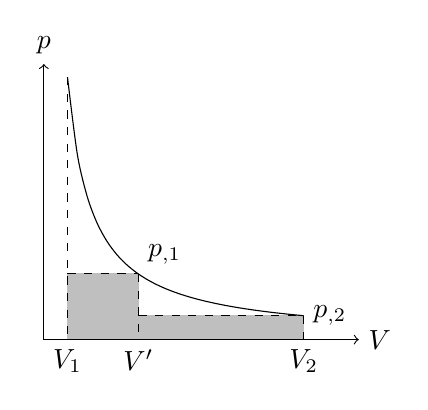
\begin{tikzpicture}
    \filldraw[lightgray] (0.3,0)--(0.3,1/1.2)--(1.2,1/1.2)--(1.2,1/3.3)--(3.3,1/3.3)--(3.3,0)--(0.3,0);
    \draw[->] (0,0) -- (4,0) node[right]{$V$};
    \draw[->] (0,0) -- (0,3.5) node[above]{$p$};
    \draw[domain=0.3:3.3] plot[smooth](\x,1/\x);
    \draw[dashed] (0.3,1/0.3) -- (0.3,0) node[below]{$V_1$};
    \draw[dashed] (3.3,1/3.3) -- (3.3,0) node[below]{$V_2$};
    \draw[dashed] (1.2,1/1.2) -- (1.2,0) node[below]{$V'$};
    \draw[dashed] (0.3,1/1.2) -- (1.2,1/1.2) node[above right]{$p_{\e,1}$};
    \draw[dashed] (1.2,1/3.3) -- (3.3,1/3.3) node[right]{$p_{\e,2}$};
\end{tikzpicture}
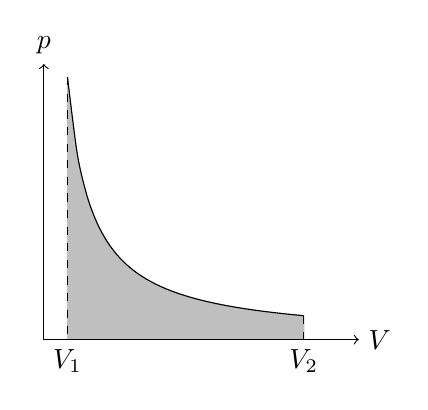
\begin{tikzpicture}
    \filldraw[lightgray] (0.3,0)--plot[domain=0.3:3.3,smooth](\x,1/\x)--(3.3,0);
    \draw[->] (0,0) -- (4,0) node[right]{$V$};
    \draw[->] (0,0) -- (0,3.5) node[above]{$p$};
    \draw[domain=0.3:3.3] plot[smooth](\x,1/\x);
    \draw[dashed] (0.3,1/0.3) -- (0.3,0) node[below]{$V_1$};
    \draw[dashed] (3.3,1/3.3) -- (3.3,0) node[below]{$V_2$};
\end{tikzpicture}
\end{document}